%%
%% First-draft workshop paper for BotXGraph.
%% Replace metadata, author affiliation, and final bibliography details as needed.
%%
\documentclass[sigconf,authordraft]{acmart}

\AtBeginDocument{%
  \providecommand\BibTeX{{%
    Bib\TeX}}}

\setcopyright{none}
\acmConference[Integrity '26]{Integrity 2026: AI-Enabled Integrity in Social Networks and Media}{August 10, 2026}{Jeju, Republic of Korea}
\acmBooktitle{Integrity 2026: AI-Enabled Integrity in Social Networks and Media, August 10, 2026, Jeju, Republic of Korea}

\usepackage{booktabs}
\usepackage{multirow}
\usepackage{url}

\title[BotXGraph]{BotXGraph: Explainable Heterogeneous Integrity Graphs for Suspicious Account Detection}

% TODO: Replace with final author metadata.
\author{Mehul Srivastava}
\affiliation{%
  \institution{Affiliation TBD}
  \country{India}}
\email{author@example.com}

\renewcommand{\shortauthors}{Srivastava}

\begin{abstract}
AI-enabled abuse has made suspicious social accounts simultaneously easier to create and harder to evaluate. Integrity teams increasingly need models that move beyond profile-only classification and instead reason over content, entities, and interaction structure, while also supporting explanation, operating-point tuning, and robustness analysis. We present BotXGraph, an explainable heterogeneous integrity-graph framework for suspicious account detection that conceptually unifies users, posts, hashtags, URLs, topics, and relations in a single graph. We then evaluate a working prototype instantiation of this broader framework on a Twitter-style bot detection setting. The current prototype combines user account features, post-text proxies, hashtag and URL nodes, and weak user-user augmentation through similarity and co-occurrence links. Empirically, the graph model reaches test macro-F1 around 0.85 and substantially higher bot recall than a stronger tabular baseline, while also enabling integrity-oriented analyses unavailable to a simple classifier. Explanation faithfulness tests show large performance drops when important relations or top-ranked features are removed; threshold tuning improves macro-F1 and precision at a different enforcement operating point; and simple AI-like profile-text perturbations degrade performance in a measurable, policy-relevant way. We argue that BotXGraph is best understood as a framework-plus-prototype contribution: a graph-native integrity design, an initial working instantiation, and an evaluation recipe for explainable suspicious-account analysis in the GenAI era.
\end{abstract}

\begin{CCSXML}
<ccs2012>
 <concept>
  <concept_id>10010147.10010257.10010293.10010294</concept_id>
  <concept_desc>Computing methodologies~Neural networks</concept_desc>
  <concept_significance>500</concept_significance>
 </concept>
 <concept>
  <concept_id>10010147.10010371.10010387.10010396</concept_id>
  <concept_desc>Computing methodologies~Reasoning about belief and knowledge</concept_desc>
  <concept_significance>300</concept_significance>
 </concept>
 <concept>
  <concept_id>10002951.10003317.10003338</concept_id>
  <concept_desc>Information systems~Social networks</concept_desc>
  <concept_significance>300</concept_significance>
 </concept>
</ccs2012>
\end{CCSXML}

\ccsdesc[500]{Computing methodologies~Neural networks}
\ccsdesc[300]{Computing methodologies~Reasoning about belief and knowledge}
\ccsdesc[300]{Information systems~Social networks}

\keywords{trust and safety, social media integrity, graph neural networks, bot detection, explainability, robustness}

\maketitle

\section{Introduction}
Social platforms now operate in an integrity environment shaped by AI on both sides of the problem. Generative models lower the cost of producing convincing personas, repetitive profile text, and coordinated narratives, while platform defenders increasingly rely on AI-assisted detection, moderation, and review operations. This creates a need for suspicious-account models that are not only accurate, but also explainable, tunable, and robust under light adversarial drift. The Integrity 2026 workshop explicitly emphasizes these themes: AI-enabled coordinated operations, synthetic personas, trust and safety tooling, and AI-enabled evaluation frameworks for robustness and harm reduction \cite{integrity2026}.

Existing suspicious-account and bot-detection pipelines often reduce the problem to a tabular profile classification task. That framing is practical, but it leaves out the contextual structure that makes integrity analysis operationally meaningful: what an account posts, which entities it repeatedly invokes, how it relates to other accounts, and which narratives or topics it inhabits. BotXGraph starts from the opposite assumption: suspicious accounts should be modeled as nodes embedded in a heterogeneous graph of content, entities, and interactions.

This paper makes four contributions. First, we formalize \emph{BotXGraph} as a heterogeneous integrity-graph framework over users, tweets, hashtags, URLs, topics, and cross-entity relations. Second, we describe a current working prototype instantiation that realizes a subset of this design using user features, text-derived post proxies, hashtag and URL nodes, and weak user-user augmentation. Third, we evaluate this prototype using integrity-oriented criteria rather than only a single aggregate score: explanation faithfulness, threshold calibration, and robustness under AI-like profile-text perturbations. Fourth, we document the limitations of the current prototype and clarify what remains to fully realize the larger architecture.

The current prototype should not be read as a full implementation of the entire BotXGraph design. Instead, it is a partial but functional realization intended to test whether graph-native suspicious-account reasoning produces operationally useful behavior. This distinction matters throughout the paper: the framework is broader than the present implementation, while the current experiments still provide substantive evidence for explainability and evaluation methodology.

\section{Related Work}
Graph-based suspicious-account detection has become increasingly important as researchers move beyond isolated account attributes toward richer relational representations. TwiBot-22 provides a large graph-oriented benchmark for Twitter bot detection and highlights the importance of diversified relations and better annotation quality \cite{feng2022twibot22}. More directly, heterogeneity-aware Twitter bot detection with relational graph transformers shows that relation-aware architectures can outperform simpler graph models when heterogeneous user relations are available \cite{feng2021relgt}. BotXGraph aligns with this line of work, but is framed less as a benchmark race and more as an integrity-analysis pipeline.

Our architecture is also inspired by work on heterogeneous graph learning and attention. Heterogeneous Graph Attention Networks (HAN) demonstrate the value of hierarchical attention over graph types \cite{wang2019han}, while KGAT highlights the usefulness of attention-based propagation over knowledge-rich relational structure \cite{wang2019kgat}. BotXGraph adopts these lessons in a task-specific way: user predictions should integrate messages from different relation types, and those relation types should remain inspectable rather than disappearing into a single flattened representation.

Explainability is especially important in trust and safety settings, where the output of a model can affect user accounts, ranking systems, or reviewer workload. Recent work on graph explanation explores hierarchical concept-based explanations \cite{jurss2023help} and structure-aware attribution mechanisms \cite{wu2025graphext}. We do not claim to implement these approaches directly. Instead, we borrow their core intuition: an integrity graph should support evidence attribution, and those attributions should be tested with faithfulness-style perturbations rather than accepted at face value.

\section{BotXGraph Framework}
\subsection{Full Intended Integrity Graph}
The full BotXGraph framework is defined over five node types and six edge types. Figure~\ref{fig:framework} shows the intended design. User nodes capture account-level metadata and aggregate behavioral cues. Tweet nodes capture textual, engagement, temporal, and language information. Hashtag and URL nodes represent narrative and coordination anchors. Topic nodes model latent thematic participation. Edges encode follows, posting, mentions, hashtag usage, URL linkage, and topic membership.

\begin{figure}[t]
  \centering
  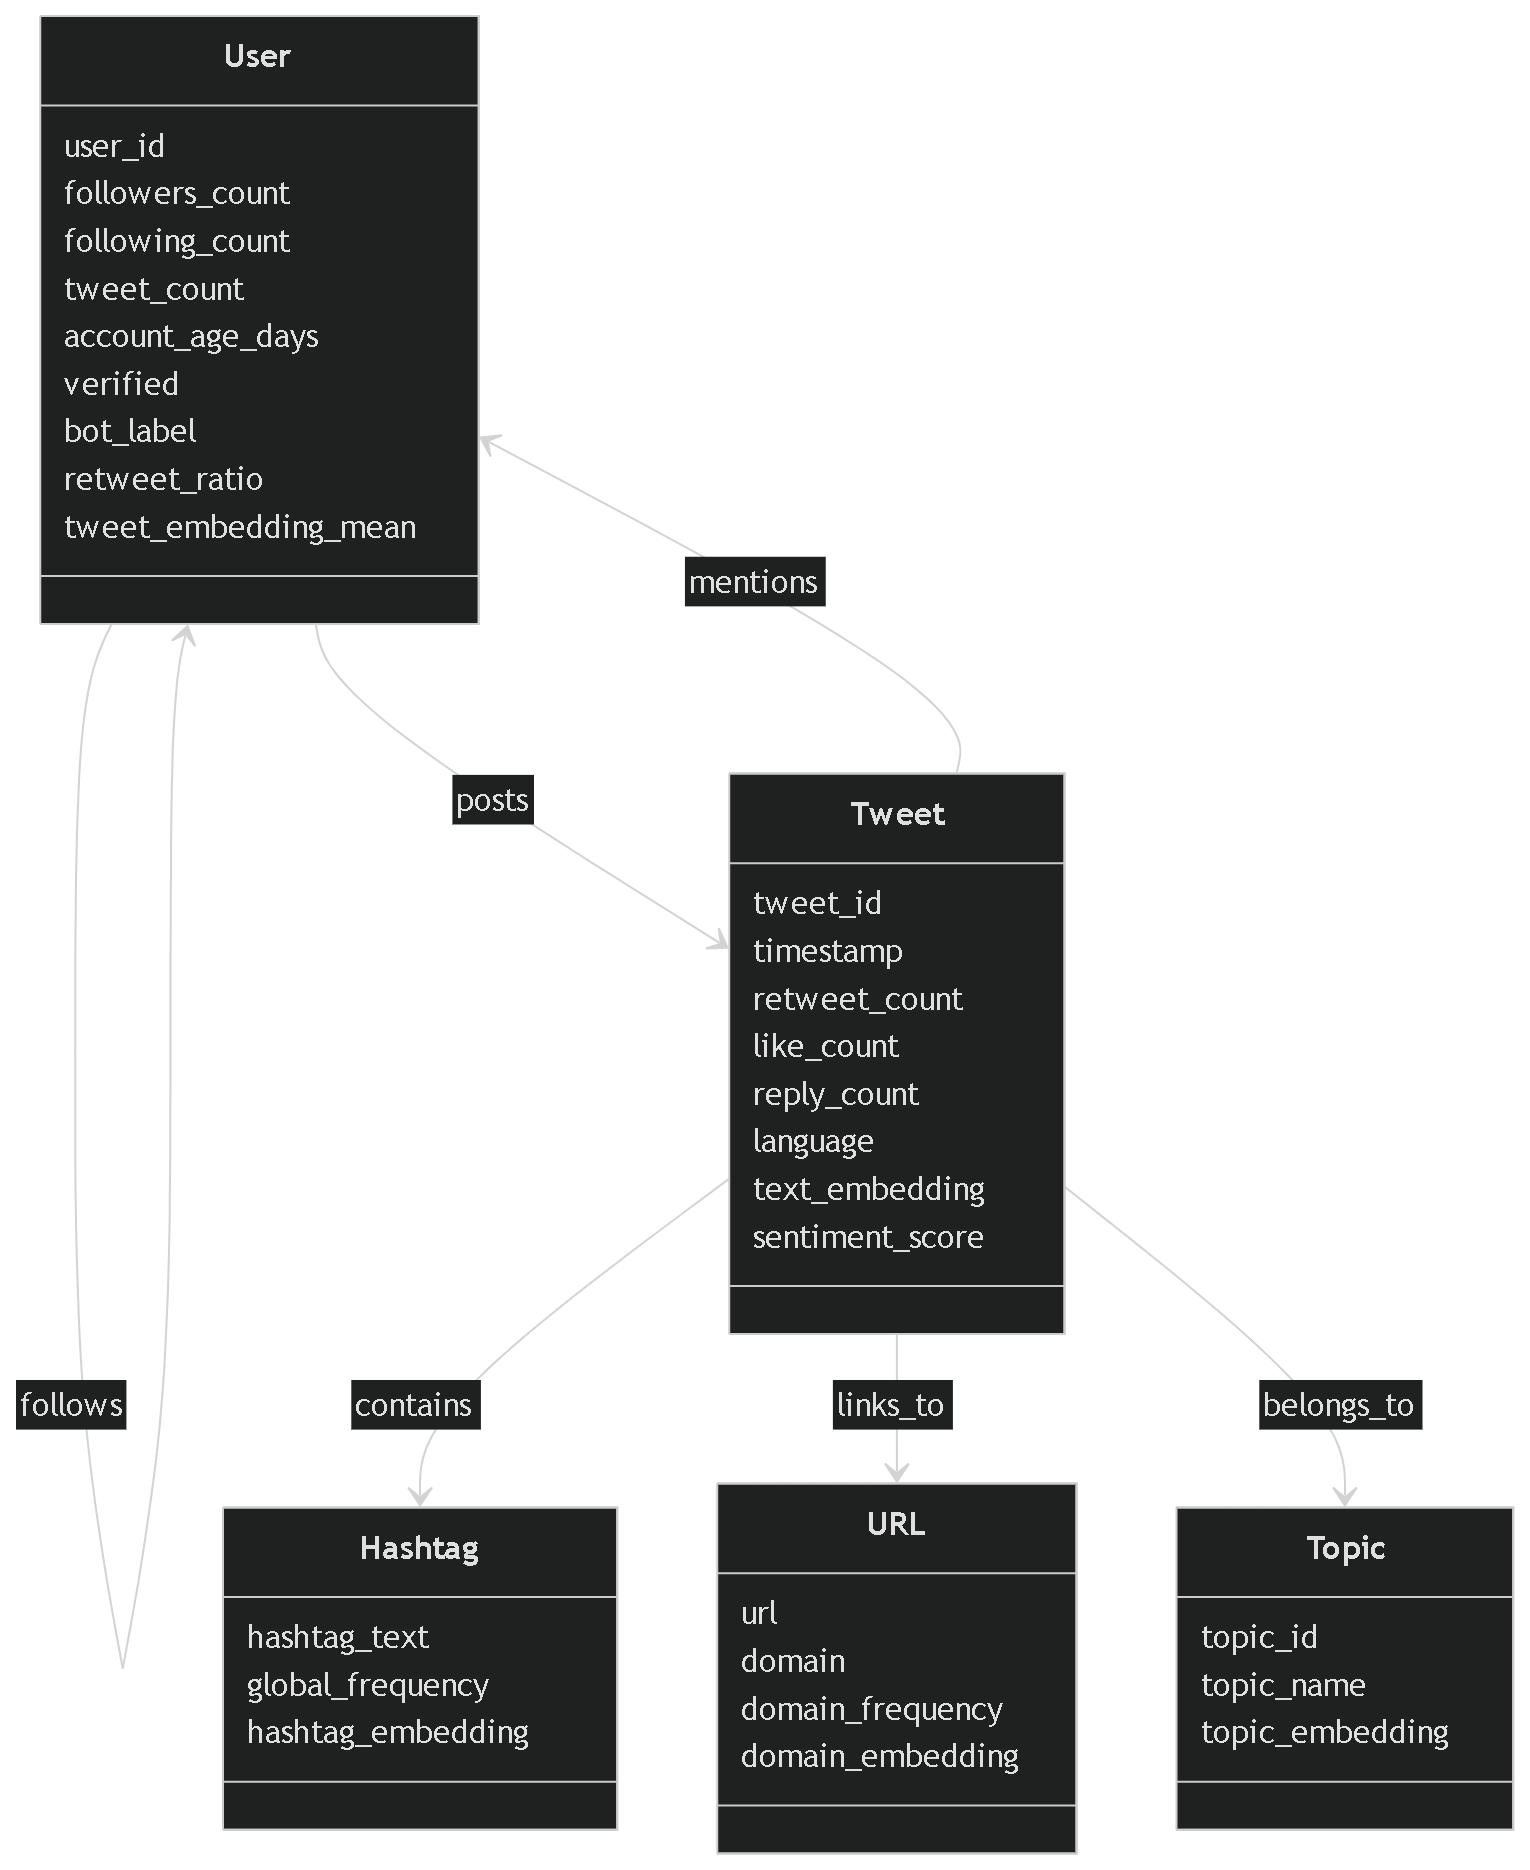
\includegraphics[width=\linewidth]{mermaid-diagram.png}
  \caption{Intended BotXGraph framework. The complete conceptual schema models users, tweets, hashtags, URLs, topics, and six relation families in a unified heterogeneous integrity graph.}
  \Description{A heterogeneous graph schema with node types User, Tweet, Hashtag, URL, and Topic, connected by follows, posts, mentions, contains, links-to, and belongs-to relations.}
  \label{fig:framework}
\end{figure}

This full graph is the \emph{framework} contribution of the paper. It is intentionally broader than the present prototype and should be understood as the target representation for graph-native suspicious-account analysis.

\subsection{Current Prototype Instantiation}
The current repository instantiates a working subset of the framework. The prototype constructs:
\begin{itemize}
\item user nodes with normalized account-level features such as followers, friends, status counts, favorites, verification, and account age;
\item tweet-proxy nodes derived from profile description text;
\item hashtag nodes extracted from text;
\item URL nodes at the domain level;
\item weak user-user relations built through profile similarity, shared hashtags, and shared URLs.
\end{itemize}

This prototype is deliberately pragmatic. The compact \texttt{twitter-human-bots} dataset provides one row per account rather than a complete native follower graph, so the implementation synthesizes a tweet proxy from profile description text and augments the graph with weak similarity and co-occurrence relations. The resulting system is not a full social graph, but it is sufficient to test whether graph-structured evidence changes detection behavior in a useful way.

\subsection{Learning Objective}
The current classifier is a relation-aware heterogeneous graph neural network that predicts the label of user nodes. Messages are aggregated separately by relation, weighted through learned attention-like importance scores, and combined with node-type-specific transformations. The present implementation also records post-hoc explanation signals:
\begin{itemize}
\item feature saliency over user attributes, using gradient-based importance;
\item relation importance, using mean contribution weights over user-directed relations.
\end{itemize}

These artifacts are central to the integrity framing of the paper. The model is useful not only if it classifies accounts, but also if it reveals which evidence channels drive those classifications and whether those channels remain stable under perturbation.

\section{Prototype Instantiation and Experimental Setup}
\subsection{Dataset and Graph Construction}
Our main experiments use the \texttt{twitter-human-bots} dataset distributed through Hugging Face \cite{twitterhumanbots}. In the current prototype, each account becomes one user node and one synthetic tweet node derived from its profile description. The resulting graph contains 37{,}438 user nodes, 37{,}438 tweet nodes, 7{,}211 hashtag nodes, and 10 URL-domain nodes. The graph includes 748{,}760 \texttt{similar\_profile} edges, 4{,}618 \texttt{co\_hashtag} edges, and 8 \texttt{co\_url} edges, in addition to user--tweet, tweet--hashtag, and tweet--URL relations.

The graph uses a 70/15/15 train/validation/test split, producing 26{,}206 training users, 5{,}616 validation users, and 5{,}616 test users. The current full-model report indicates that tweet text was encoded with a TF-IDF plus SVD fallback encoder rather than a transformer model in the reported run.

\subsection{Models and Metrics}
We compare two main systems:
\begin{itemize}
\item a fast baseline using the user-level feature set without heterogeneous message passing;
\item the BotXGraph prototype, a relation-aware heterogeneous GNN over the instantiated graph.
\end{itemize}

We report accuracy, macro-F1, bot precision, and bot recall. We deliberately emphasize bot recall in discussion because suspicious-account triage often prefers not to miss risky accounts, even when overall macro-F1 is not maximal.

\subsection{Integrity-Oriented Evaluation}
In addition to the baseline comparison, the repository includes three completed integrity-oriented evaluations that are already usable in the paper:
\begin{itemize}
\item \textbf{Faithfulness}: remove high-importance relations or top-ranked user features and measure performance and probability shift.
\item \textbf{Threshold sweep}: change the bot decision threshold and evaluate alternate enforcement operating points.
\item \textbf{Robustness}: perturb profile-text content with light rewrites, hashtag injection, URL injection, and a combined attack.
\end{itemize}

Two additional expensive evaluations were started but interrupted by a server disconnect:
\begin{itemize}
\item \textbf{Multi-seed stability}: intended over five seeds, partially completed for two seeds.
\item \textbf{Ablation study}: intended over six graph variants, partially completed for three variants.
\end{itemize}

\section{Results}
\subsection{Main Performance and Operational Tradeoffs}
Table~\ref{tab:main-results} summarizes the core detection results already available in the repository. The fast baseline is stronger on aggregate test accuracy and macro-F1, whereas the BotXGraph prototype substantially improves bot recall. This is the first key framing decision for the paper: the graph model should not be sold as an across-the-board winner, but as a model that shifts the operating point toward recall and interpretable evidence integration.

\begin{table}[t]
  \caption{Main performance comparison on the \texttt{twitter-human-bots} prototype setting.}
  \label{tab:main-results}
  \begin{tabular}{lcccc}
    \toprule
    Model & Accuracy & Macro-F1 & Bot Prec. & Bot Rec. \\
    \midrule
    Baseline & 0.8803 & 0.8605 & 0.8643 & 0.7586 \\
    BotXGraph prototype & 0.8634 & 0.8493 & 0.7698 & 0.8396 \\
    \bottomrule
  \end{tabular}
\end{table}

The full-model explanation snapshot also offers useful qualitative evidence. The most salient user features are \texttt{log1p\_favourites\_count}, \texttt{log1p\_followers\_count}, and \texttt{average\_tweets\_per\_day}. The most important user-directed relations are \texttt{tweet\_\_rev\_posts\_\_user}, \texttt{similar\_profile}, and \texttt{co\_hashtag}. Figure~\ref{fig:rel-importance} shows one of the generated relation-importance plots already present in the repository.

\begin{figure}[t]
  \centering
  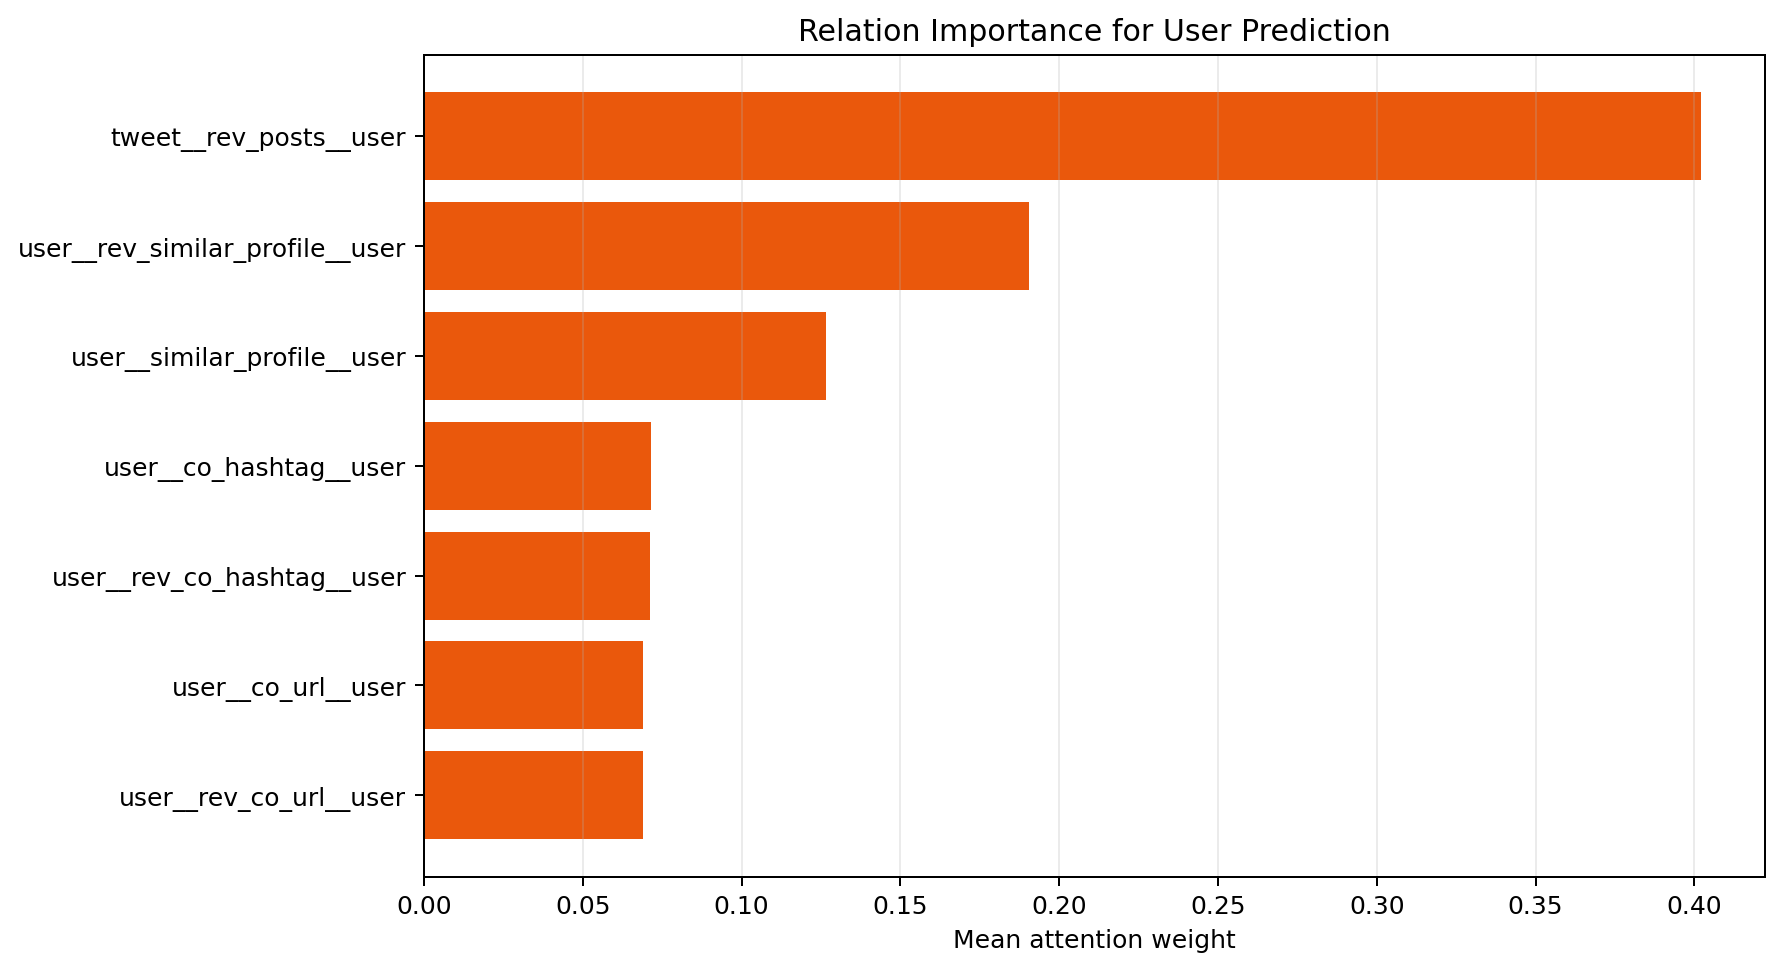
\includegraphics[width=\linewidth]{reports/plots/hetero_gnn_full/relation_importance.png}
  \caption{Relation importance from the full BotXGraph prototype run. Posting/text linkage and profile-similarity structure dominate the current instantiation.}
  \Description{A horizontal bar chart ranking relation importance for user prediction, with tweet-to-user posting and profile-similarity relations contributing most.}
  \label{fig:rel-importance}
\end{figure}

\subsection{Explanation Faithfulness}
Table~\ref{tab:faithfulness} summarizes the completed faithfulness experiment. Removing either the top user features or the \texttt{similar\_profile} relation causes large, measurable degradation. This provides concrete support for the claim that BotXGraph explanations are not purely decorative. The model is genuinely using the evidence it highlights.

\begin{table*}[t]
  \caption{Faithfulness results on the completed full-model run.}
  \label{tab:faithfulness}
  \begin{tabular}{lccccc}
    \toprule
    Perturbation & Accuracy & Macro-F1 & Bot Precision & Bot Recall & Mean Abs.\ Prob.\ Shift \\
    \midrule
    Full graph & 0.8636 & 0.8495 & 0.7699 & 0.8401 & 0.0000 \\
    Drop \texttt{similar\_profile} & 0.8095 & 0.7689 & 0.7836 & 0.5885 & 0.1179 \\
    Drop hashtag and URL edges & 0.8339 & 0.8222 & 0.7014 & 0.8696 & 0.0665 \\
    Mask top 3 user features & 0.7425 & 0.6888 & 0.6474 & 0.4925 & 0.1993 \\
    \bottomrule
  \end{tabular}
\end{table*}

Two patterns matter here. First, profile similarity is a major structural signal in the current prototype: dropping it sharply reduces bot recall from 0.8401 to 0.5885. Second, removing hashtag and URL evidence does not simply collapse the classifier; instead, it shifts the precision--recall balance, reducing precision while increasing recall. This is exactly the kind of integrity-relevant nuance that a graph model can surface.

The repository also contains complementary visualizations in \texttt{reports/paper\_experiments/faithfulness/faithfulness\_metric\_drop.png} and \texttt{faithfulness\_probability\_shift.png}, which can be used directly or moved to an appendix if space is tight.

\subsection{Threshold Calibration}
The threshold sweep demonstrates that a fixed 0.50 decision threshold is not necessarily the right operating point. Validation-based tuning selects 0.60 as the best threshold by validation macro-F1. Table~\ref{tab:threshold} shows the resulting shift in performance, and Figure~\ref{fig:threshold} visualizes the test-time tradeoff curve.

\begin{table}[t]
  \caption{Threshold sweep summary for the completed BotXGraph run.}
  \label{tab:threshold}
  \begin{tabular}{lcccc}
    \toprule
    Threshold & Accuracy & Macro-F1 & Bot Prec. & Bot Rec. \\
    \midrule
    0.50 (default) & 0.8627 & 0.8488 & 0.7670 & 0.8423 \\
    0.60 (tuned) & 0.8722 & 0.8553 & 0.8121 & 0.7999 \\
    \bottomrule
  \end{tabular}
\end{table}

\begin{figure}[t]
  \centering
  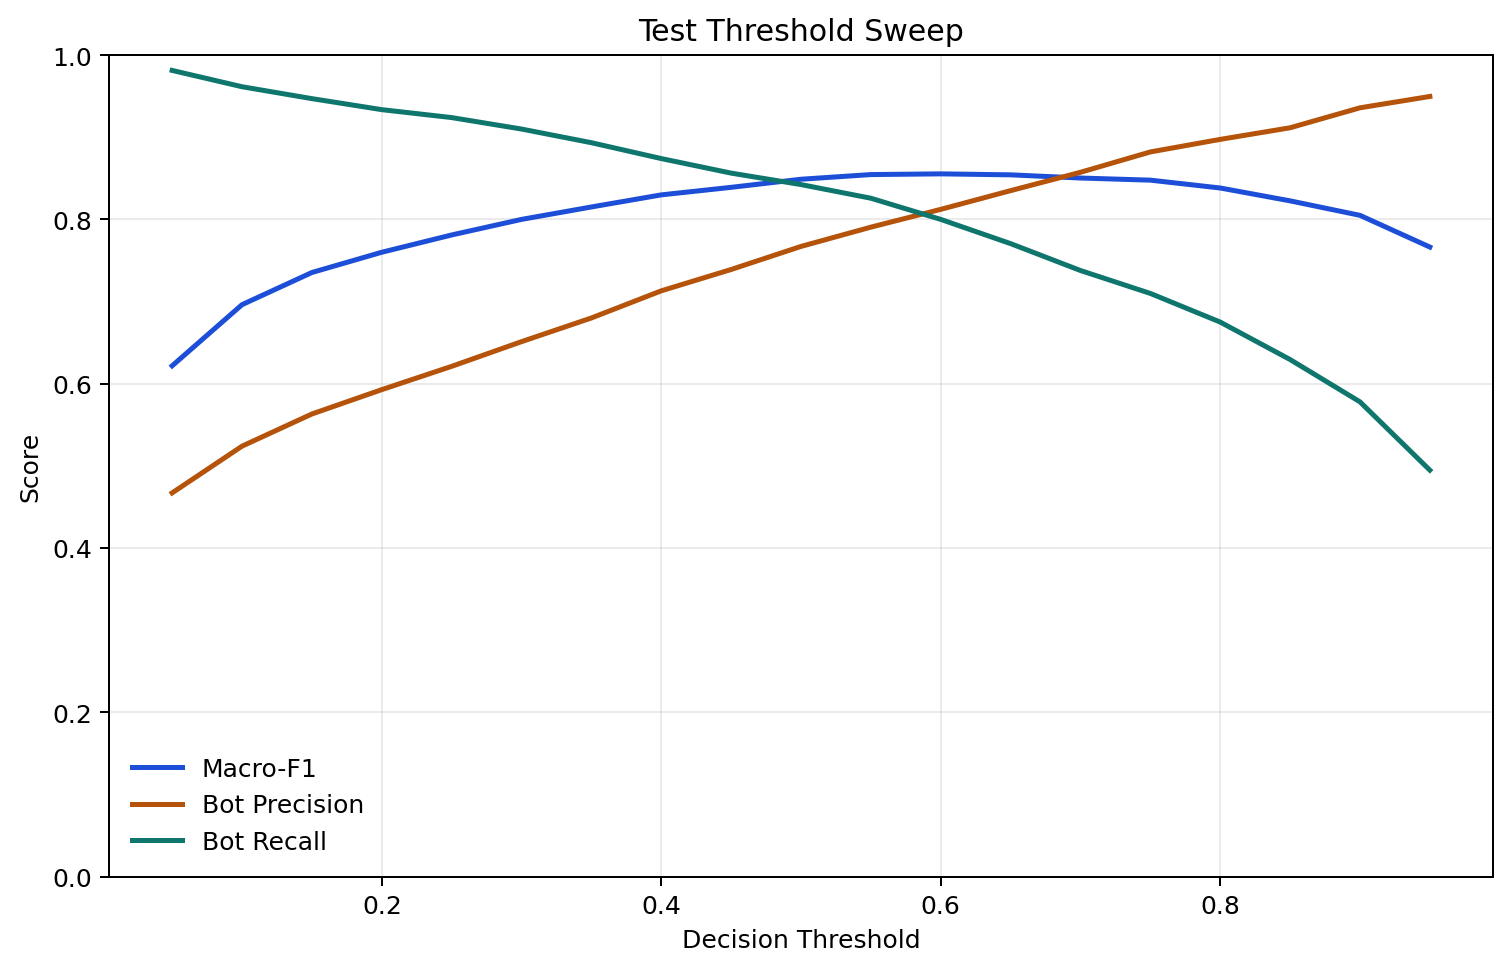
\includegraphics[width=\linewidth]{reports/paper_experiments/threshold/test_threshold_curves.png}
  \caption{Threshold sweep on the completed test run. Precision, recall, and macro-F1 move along a meaningful operating frontier rather than concentrating at the default threshold.}
  \Description{A line plot of threshold versus macro-F1, bot precision, and bot recall. Macro-F1 peaks around a threshold of 0.60.}
  \label{fig:threshold}
\end{figure}

This result is highly relevant to trust and safety. Different platforms or product surfaces may prefer different operating points depending on reviewer capacity, downstream enforcement friction, or the cost of false positives. BotXGraph is therefore better understood as a decision-support model than as a one-threshold detector.

\subsection{Robustness to AI-like Profile-Text Perturbations}
Robustness results in Table~\ref{tab:robustness} show that the current prototype is measurably sensitive to profile-text perturbations. Macro-F1 drops from 0.8485 in the clean setting to 0.8033--0.8198 across the tested perturbations, with non-trivial changes in prediction confidence.

\begin{table*}[t]
  \caption{Robustness results under simple AI-like profile-text perturbations.}
  \label{tab:robustness}
  \begin{tabular}{lccccc}
    \toprule
    Perturbation & Accuracy & Macro-F1 & Bot Precision & Bot Recall & Mean Abs.\ Prob.\ Shift \\
    \midrule
    Clean & 0.8625 & 0.8485 & 0.7676 & 0.8401 & 0.0000 \\
    Light rewrite & 0.8275 & 0.8095 & 0.7208 & 0.7838 & 0.0889 \\
    Hashtag injection & 0.8264 & 0.8033 & 0.7433 & 0.7285 & 0.1111 \\
    URL injection & 0.8316 & 0.8112 & 0.7406 & 0.7580 & 0.0889 \\
    Combined attack & 0.8413 & 0.8198 & 0.7686 & 0.7468 & 0.0910 \\
    \bottomrule
  \end{tabular}
\end{table*}

This is not a negative result; it is a useful one. The completed robustness outputs show that the current BotXGraph instantiation is sensitive to relatively simple text-level manipulations, which makes robustness itself a first-class integrity evaluation target rather than an afterthought. Figure~\ref{fig:robustness} provides the generated plot already available in the repository.

\begin{figure}[t]
  \centering
  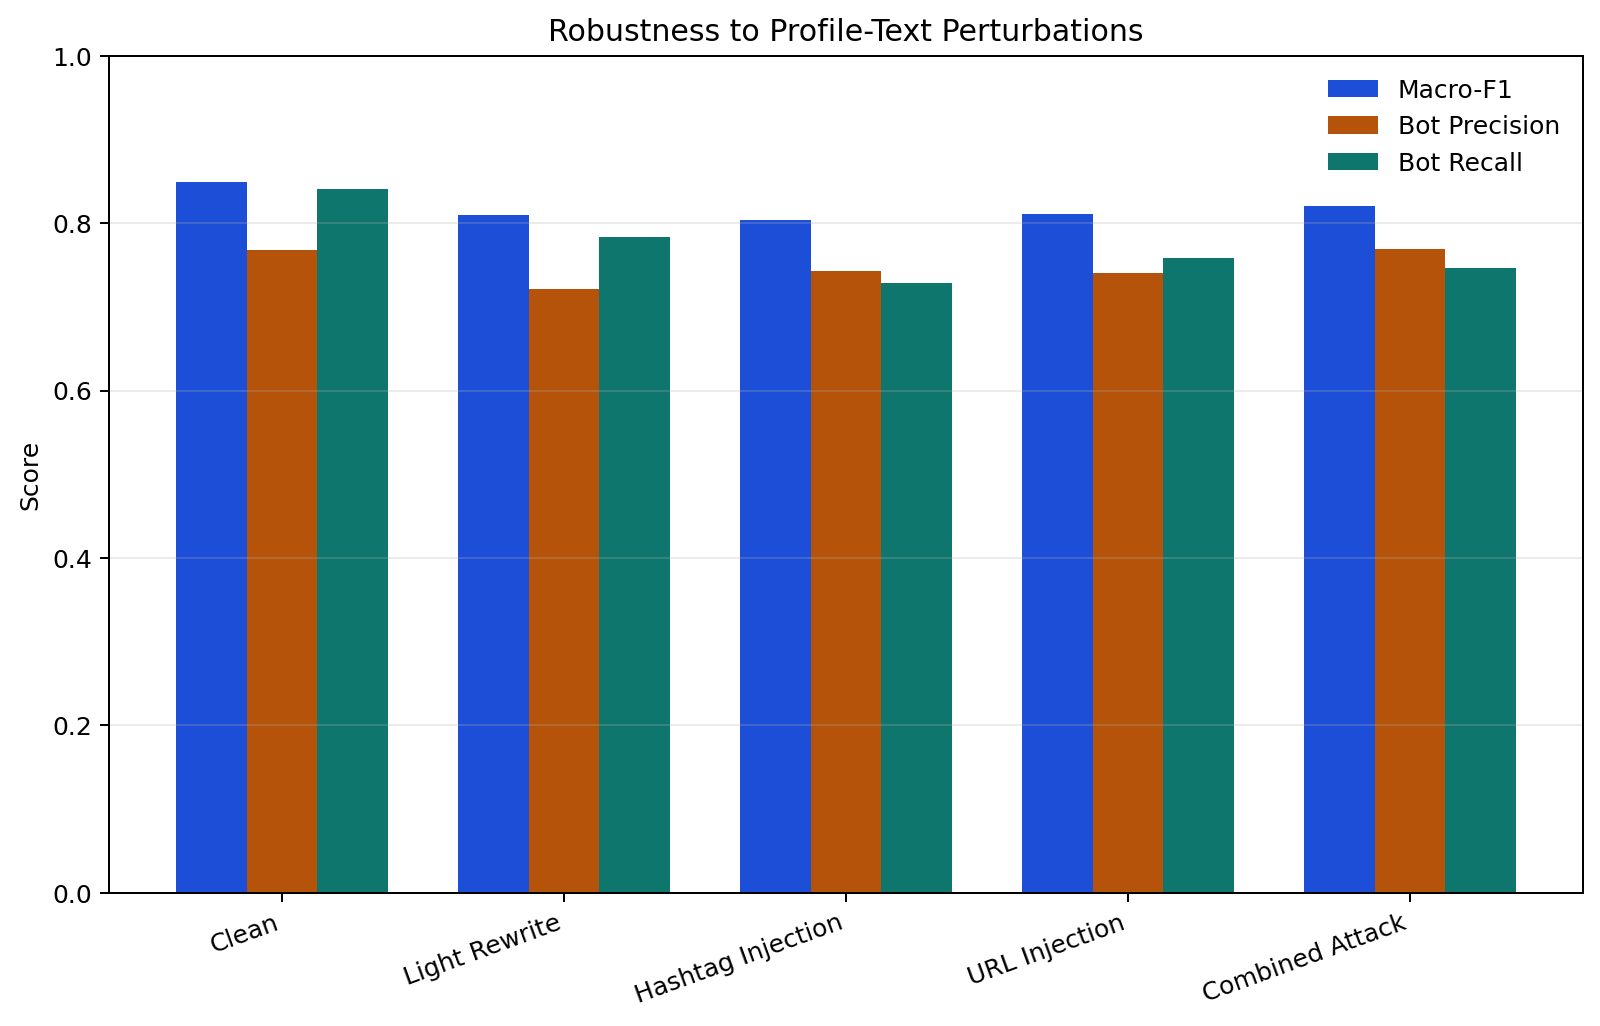
\includegraphics[width=\linewidth]{reports/paper_experiments/robustness/robustness_metrics.png}
  \caption{Robustness metrics under AI-like profile-text perturbations. The current prototype remains informative, but performance declines are clearly measurable.}
  \Description{A grouped bar chart comparing test macro-F1, bot precision, and bot recall under clean, rewrite, hashtag injection, URL injection, and combined perturbations.}
  \label{fig:robustness}
\end{figure}

\subsection{Preliminary Ongoing Analyses}
Two heavier experiment families were interrupted by a server disconnect and remain incomplete at the time of this draft. We still note their partial outputs because they are directionally informative:
\begin{itemize}
\item \textbf{Partial multi-seed results:} seed 42 reached macro-F1 0.8500 and seed 43 reached macro-F1 0.8428 before the run stopped during seed 44.
\item \textbf{Partial ablation results:} \texttt{profile\_only} reached macro-F1 0.8442, \texttt{profile\_plus\_text} reached 0.8474, and \texttt{plus\_similar\_profile} reached 0.8492 before the run stopped during \texttt{plus\_co\_hashtag}.
\end{itemize}

These preliminary numbers already suggest that profile-only performance is strong, text adds a modest gain, and profile-similarity augmentation adds another incremental gain. However, because the full ablation and multi-seed analyses are not finished, they should be treated as ongoing rather than final evidence.

\section{Discussion}
The completed results support three main claims. First, BotXGraph is a useful framework for \emph{operational evaluation}, even when its current prototype does not dominate a strong tabular baseline on macro-F1. Faithfulness, threshold calibration, and robustness all reveal behavior that would remain invisible in a pure profile-only classifier. Second, the present instantiation appears to rely heavily on user features and profile-similarity augmentation. This is both a strength and a limitation: it provides a strong weak-graph signal, but it also means that the current implementation is still some distance away from the richer full framework with follows, mentions, and topics. Third, threshold and perturbation analyses make the prototype much more aligned with trust and safety practice than a one-number benchmark paper would be.

The broader lesson is that graph-native suspicious-account reasoning should not be judged only by whether it wins a single accuracy table. A richer graph representation is valuable if it offers better integrity tradeoffs, clearer evidence attribution, and a more realistic evaluation protocol for AI-enabled abuse settings.

\section{Limitations and Future Work}
This draft intentionally distinguishes between the \emph{framework} and the \emph{current prototype}. The full BotXGraph design includes follower structure, mentions, topic nodes, and richer interaction semantics that are not fully realized in the present code. The main dataset used here is also limited: it provides a compact account-level benchmark rather than a full native social graph. As a consequence, the prototype constructs tweet proxies from profile descriptions and relies heavily on weak similarity and co-occurrence edges.

The robustness tests are also controlled rather than fully adaptive. They are useful integrity probes, but they do not approximate a strategic adversary with access to model feedback. Finally, the multi-seed and ablation studies were partially interrupted and therefore remain incomplete in this draft. Completing those runs, along with a second dataset instantiation such as TwiBot-22, would substantially strengthen the stability and portability claims.

\section{Conclusion}
We presented BotXGraph as a framework-plus-prototype contribution for suspicious-account integrity analysis. The full framework proposes a heterogeneous graph over users, posts, hashtags, URLs, topics, and cross-entity relations. The current repository implements a working prototype instantiation that already supports graph-based user classification, feature and relation explanation, threshold calibration, and perturbation robustness analysis. The resulting paper should not be read as a state-of-the-art performance claim. Instead, it argues that explainable integrity graphs are a useful direction for AI-enabled trust and safety: they expose evidence pathways, support operational threshold choices, and provide a more realistic evaluation lens for suspicious-account systems in the GenAI era.

\begin{acks}
This first draft uses placeholder metadata and a draft bibliography. Final author details, acknowledgments, and any institutional or funding disclosures should be added before submission.
\end{acks}

\bibliographystyle{ACM-Reference-Format}
\bibliography{botxgraph_refs}

\appendix

\section{Available Generated Outputs in the Repository}
The repository already contains several paper-ready plots and summaries that can be selectively included or moved to supplementary material:
\begin{itemize}
\item \texttt{reports/plots/hetero\_gnn\_full/training\_curves.png}
\item \texttt{reports/plots/hetero\_gnn\_full/edge\_type\_counts.png}
\item \texttt{reports/plots/hetero\_gnn\_full/confusion\_matrix.png}
\item \texttt{reports/plots/hetero\_gnn\_full/feature\_saliency.png}
\item \texttt{reports/plots/hetero\_gnn\_full/relation\_importance.png}
\item \texttt{reports/plots/hetero\_gnn\_full/graph\_schema.png}
\item \texttt{reports/plots/hetero\_gnn\_full/user\_projection.png}
\item \texttt{reports/plots/hetero\_gnn\_full/similarity\_subgraph.png}
\item \texttt{reports/paper\_experiments/faithfulness/faithfulness\_metric\_drop.png}
\item \texttt{reports/paper\_experiments/faithfulness/faithfulness\_probability\_shift.png}
\item \texttt{reports/paper\_experiments/threshold/val\_threshold\_curves.png}
\item \texttt{reports/paper\_experiments/threshold/test\_threshold\_curves.png}
\item \texttt{reports/paper\_experiments/robustness/robustness\_metrics.png}
\item \texttt{reports/paper\_experiments/robustness/robustness\_probability\_shift.png}
\end{itemize}

\section{Partial Interrupted Runs}
The following results exist in partially completed form and may be used for internal context, but they should not be treated as finalized unless the interrupted runs are repeated:
\begin{itemize}
\item \textbf{Multi-seed:} completed seeds 42 and 43; seed 44 interrupted; seeds 45 and 46 not completed.
\item \textbf{Ablations:} completed \texttt{profile\_only}, \texttt{profile\_plus\_text}, and \texttt{plus\_similar\_profile}; interrupted during \texttt{plus\_co\_hashtag}; \texttt{plus\_co\_url} and \texttt{full} not completed.
\end{itemize}

\end{document}
